    %
    { \footnotesize
    \begin{figure}
    \centering
    %
    \begin{subfigure}{.45\textwidth}
        $
        \begin{array}{l}
            N < m < n\\
            \kw{threeNestedWhile}(n, m, N) \triangleq \\
            \clabel{ \assign{i}{0} }^{0} ; \\
                L_1: \ewhile ~ \clabel{i < n}^{1} ~ \edo ~ \\
                \quad \Big(
                 \highlight{\clabel{\assign{j}{0}}^{2}} ;\\
                 L_3:  \quad \ewhile ~ \clabel{j < m}^{3} ~ \edo ~ \\
                \quad \quad \Big( \clabel{\assign{j}{j+1}}^{4};\\
                  \quad \quad \highlight{\clabel{\assign{w}{i}}^{5}};\\
                  L_6:  \quad \quad \ewhile ~ \clabel{w < N}^{6} ~ \edo ~ \\
                  \quad \quad \quad \Big( \clabel{\assign{w}{w + 1}}^{7}
                      \Big); \\
                      \quad \quad \clabel{\assign{i}{w}}^{8}
                      \Big); \\
                      \quad \clabel{\assign{i}{i+1}}^{9}
                  \Big)
            \end{array}
            $
    \caption{}
        \end{subfigure}
    \begin{subfigure}{.45\textwidth}
        \begin{centering}
            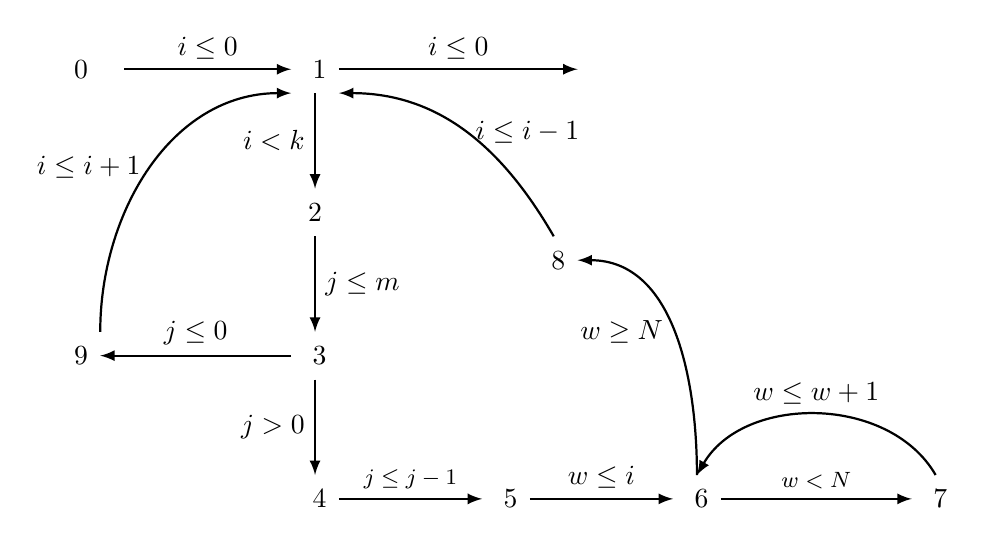
\begin{tikzpicture}[scale=\textwidth/20cm,samples=200]
                \draw[] (-5, 10) circle (0pt) node{{ $0$}};
                \draw[] (0, 10) circle (0pt) node{{ $1$}};
                \draw[] (6, 10) circle (0pt) node {{$\lex$}};
                \draw[] (0, 7) circle (0pt) node{{$2$}};
                \draw[] (0, 4) circle (0pt) node{{ $3$}};
                \draw[] (-5, 4) circle (0pt) node{{ $9$}};
                \draw[] (0, 1) circle (0pt) node{{ $4$}};
                \draw[] (4, 1) circle (0pt) node{{ $5$}};
                \draw[] (8, 1) circle (0pt) node{{ $6$}};
                \draw[] (13, 1) circle (0pt) node{{ $7$}};
                \draw[] (5, 6) circle (0pt) node{{ $8$}};
                % Counter Variables
                %
                % Control Flow Edges:
                \draw[ thick, -latex] (-4, 10)  -- node [above] {$i \leq 0$}(-0.5, 10);
                \draw[ thick, -latex] (0, 9.5)  -- node [left] {$i < k$} (0, 7.5) ;
                \draw[ thick, -latex] (0, 6.5)  -- node [right] {$j \leq m$} (0, 4.5) ;
                \draw[ thick, -latex] (0, 3.5)  -- node [left] {$j > 0$} (0, 1.5) ;
                \draw[ thick, -latex] (-0.5, 4)  -- node [above] {$j \leq 0$} (-4.5, 4) ;
                \draw[ thick, -latex] (-4.5, 4.5)  to  [out=90,in=180]  node [left] {$i \leq i + 1$ }(-0.5, 9.5);
                \draw[ thick, -latex] (0.5, 10)  -- node [above] {$i \leq 0$}  (5.5, 10);
                \draw[ thick, -latex] (0.5, 1)  -- node [above] {{\footnotesize $j \leq j - 1$}}  (3.5, 1);
                \draw[ thick, -latex] (4.5, 1)  -- node [above] {$w \leq i$}  (7.5, 1);
                \draw[ thick, -latex] (8.5, 1)  -- node [above] {{\footnotesize $w < N$}}  (12.5, 1);
                \draw[ thick, -latex] (8, 1.5)  to [out=90,in=0] node [left] {{$w \geq N$}}  (5.5, 6);
                \draw[ thick, -latex] (13, 1.5)  to  [out=120,in=60] node [above] {$w \leq w + 1$}  (8, 1.5);
                \draw[ thick, -latex] (5, 6.5)  to  [out=120,in=0]  node [right] {$i \leq i - 1$ }(0.5, 9.5);
                \end{tikzpicture}
%     \caption{}
%     \end{centering}
%     \end{subfigure}
% \begin{subfigure}{.2\textwidth}    
% \begin{centering}
    $
    \begin{array}{l}
        \tpath_0 = (0 \to 1)
        \\
        \tpath_1 = (1 \to 2 \to 3)
        \\        
        \tpath_2 = (3 \to 4 \to 5 \to 6)
        \\
        \tpath_3 = (6 \to 7 \to 6)
        \\
        \tpath_6 = (1 \to \lex)
        \\
        \tpath_4 = (6 \to 8 \to 3)
        \\
        \tpath_5 = (3 \to 9 \to 1)
    \end{array}
$
\caption{}
\end{centering}
\end{subfigure}
    \caption{
    (a) An example of three nested loops with related iterator variables.
    (b) The abstract transition graph and simple transition paths.}
        \label{fig:threeWhile-overview}
    \end{figure}
    }